\section{Grafické prvky}\label{analyza-graficke-prvky}

Pro zvýšení použitelnosti a přehlednosti jsem se rozhodl do aplikace zakomponovat grafické prvky (ikony tlačítek, zobrazovaná varování, \ldots).
Protože cílím aplikaci nejen na iPhone, ale i na iPad, musí veškerá zakomponovaná grafika být ve vysokém rozlišení.
Jednotlivé ikony a obrázky lze do Xcode nahrát pomocí \textit{Assets catalog}, tedy galerie obrázků.
Jako alternativní možnost jsem se rozhodl zanalyzovat knihovnu \textit{Iconic}, která umožňuje využít grafických fontů.

\subsection{Assets catalog}

Assets catalog je galerie obrázků přímo integrovaná do vývojového prostředí Xcode a grafického frameworku UIKit \cite{apple-xcode-assets-catalog}.
Obrázky se do galerie přidávají v různých velikostech (pro různou hustotu pixelů na displayi), typicky v rozlišení 1:1, 2:1 a 3:1.
Správa různých velikostí je vidět na obrázku \ref{fig:xcode-assets-catalog}
V aplikaci se následně přistupuje k obrázku podle jeho jména, systém sám rozhodne jakou veliost využít aby na displayi vypadala nejlépe.

\begin{figure}\centering
	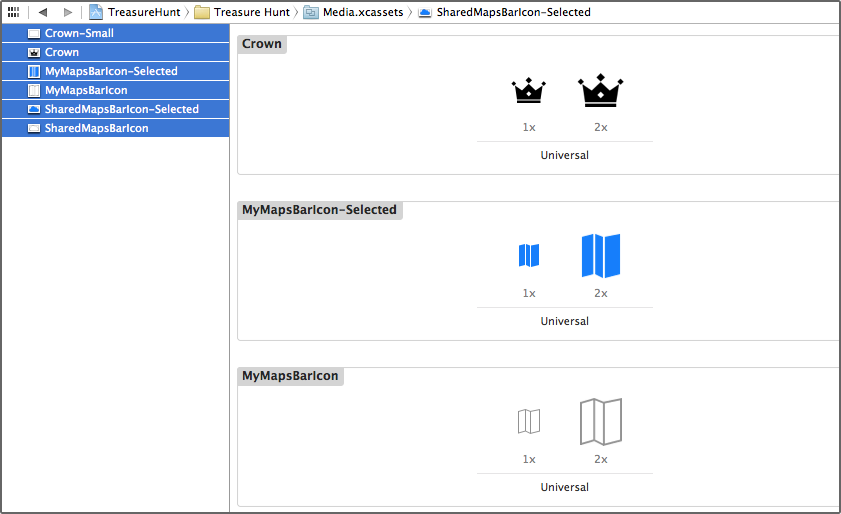
\includegraphics[width=\textwidth]{assets/analysis-graphics-assets-catalog.png}
	\caption{Assets catalog v Xcode IDE \cite{rw-update-app-for-ios7}}\label{fig:xcode-assets-catalog}
\end{figure}

S roustoucím počtem obrázků se ale dramaticky snižuje přehlednost galerie i naopak roste velikost aplikace.

\subsection{Iconic}

Alternativní metodou k Assets catalog jsou grafické fonty.
Ty mají výhodu v tom, že jsou obsažené v jednom souboru a jsou vektorové.
Pokud tedy přijde zařízení s ještě větší hustotou pixelů než existují dnes, nebude potřeba obrázky znovu exportovat, vše bude fungovat automaticky.
V současné době jediným frameworkem převádějícím fontové znaky na obrázky je Iconic.
Iconic rozparsuje zadaný font a vytvoří pro něj výčtový typ v jazyku Swift.
Pomocí výčtového typu lze pak k obrázkům přistupovat pomocí jejich jména, kde navíc platnost jména ověřuje kompilátor.
Protože se fonty typicky generují na začátku tvoření aplikace, pouští se Iconic typicky jen jednou a jeho výstup včetně fontu se následně přidává do projektu.

Pro obdobné použití jako s Assets catalog nabízí Iconic rozšíření frameworku UIKit.
Tyto rozšíření umožňují využívat fonty nejen ve zdrojovém kódu, ale i v \textit{Interface builder} rozhraní.
Využití v kódu je naznačené v ukázce \ref{code:iconic-fonts}.

\swiftcode{code:iconic-fonts}{Využití grafického fontu s frameworkem Iconic}{assets/code/iconic-fonts.swift}

Oproti Assets catalog ale postrádá možnost cachování \cite{github-iconic-cache}.
Bude-li tedy na obrazovce velké množství stejných obrázků nebo budou-li se často překreslovat, mohl by vzniknout problém s výkonem aplikace.
